\chapter{Feature Design} \label{sec:feature}

% Chapter overview of sections
% Chapter overview of sections
% Chapter overview of sections

% Introduction into sections
\section{System Overview}

\paragraph{What is OASIS}
% What is OASIS
% What is your objective with oasis
The online architectural sketching interface for simulations (OASIS) is intended to be a  general early design tool for both novices and architects. OASIS provides a platform independent sketching interface that generates closed 3D triangle meshes with optimal properties for simulations. Currently, OASIS only supports daylighting visualizations; however, OASIS can be extended to support other simulations that make use of closed triangle meshes, including acoustic and thermal simulations. The main advantage OASIS offers users is an novel interface that does not require detailed geometric modeling for the creation of 3D triangle meshes and an interface to analyze simulation results. An additional advantage of using OASIS is the client-server architecture that allows users to be able to run computationally expensive simulations at interactive rates regardless of their machine specifications.

\paragraph{Virtual Heliodon Pipeline}
% <Pipeline of the Virtual Heliodon>
Both OASIS and the Virtual Heliodon provide a novel solution to the challenge of daylighting analysis during the early stage of architectural design.
In addition to sharing the same objectives both OASIS and the Virtual Heliodon utilize the physical sketch interpretation algorithm and the daylight rendering engine.
As a result it can be difficult to see where these two systems vary.
In order to understand the contributions I made to OASIS we must briefly cover the system pipeline of the Virtual Heliodon.
The Virtual Heliodon's system pipeline is illustrated in Figure-\ref{fig:pipeline_vh}.
To begin, the Virtual Heliodon features a novel tangible user interface for the creation of architectural spaces.
Users define architectural spaces by manipulating physical foam primitives with their hands.
After users are satisfied with their architectural space they can either use a wireless clicker or communicate to the operator to run the \textit{table top detect} process and continue to generate a closed triangle mesh from their physical sketches; Communication with the operator to run the \textit{table top detect} process is noted in Figure-\ref{fig:pipeline_vh}A.
The \textit{table top detect} processes is a simple computer vision program that takes an overhead image of the foam primitives and detects where those primitives are in an image.
The coordinates of where those primitives are in an image are stored in an intermediate primitives file. The intermediate primitives file is used as input for the physical sketch interpretation algorithm. As mentioned previously, the physical sketch interpretation algorithm generates a closed watertight triangle mesh.
Currently, there exist no user interface for the generation of daylight visualizations.
Instead, an operator familiar with the system is required to generate visualizations for users, as shown in Figure-\ref{fig:pipeline_vh}B.
After the generation of  a watertight 3D mesh, users communicate to the operator the time and date they would like visualized. 
Depending on the time,date, and user visualization requested the operator would manually modify existing scripts to generate those visualizations on the Virtual Heliodon.
These scripts would include invoking the daylight rendering engine to generate image textures to be projected onto users' physical sketches.
In other words, the Virtual Heliodon does not offer much autonomy and requires an operator to both explain how to use the tangible user interface and constantly communicate with users to operate the Virtual Heliodon.
% </Pipeline of the Virtual Heliodon>

\begin{figure}[h]
\centering
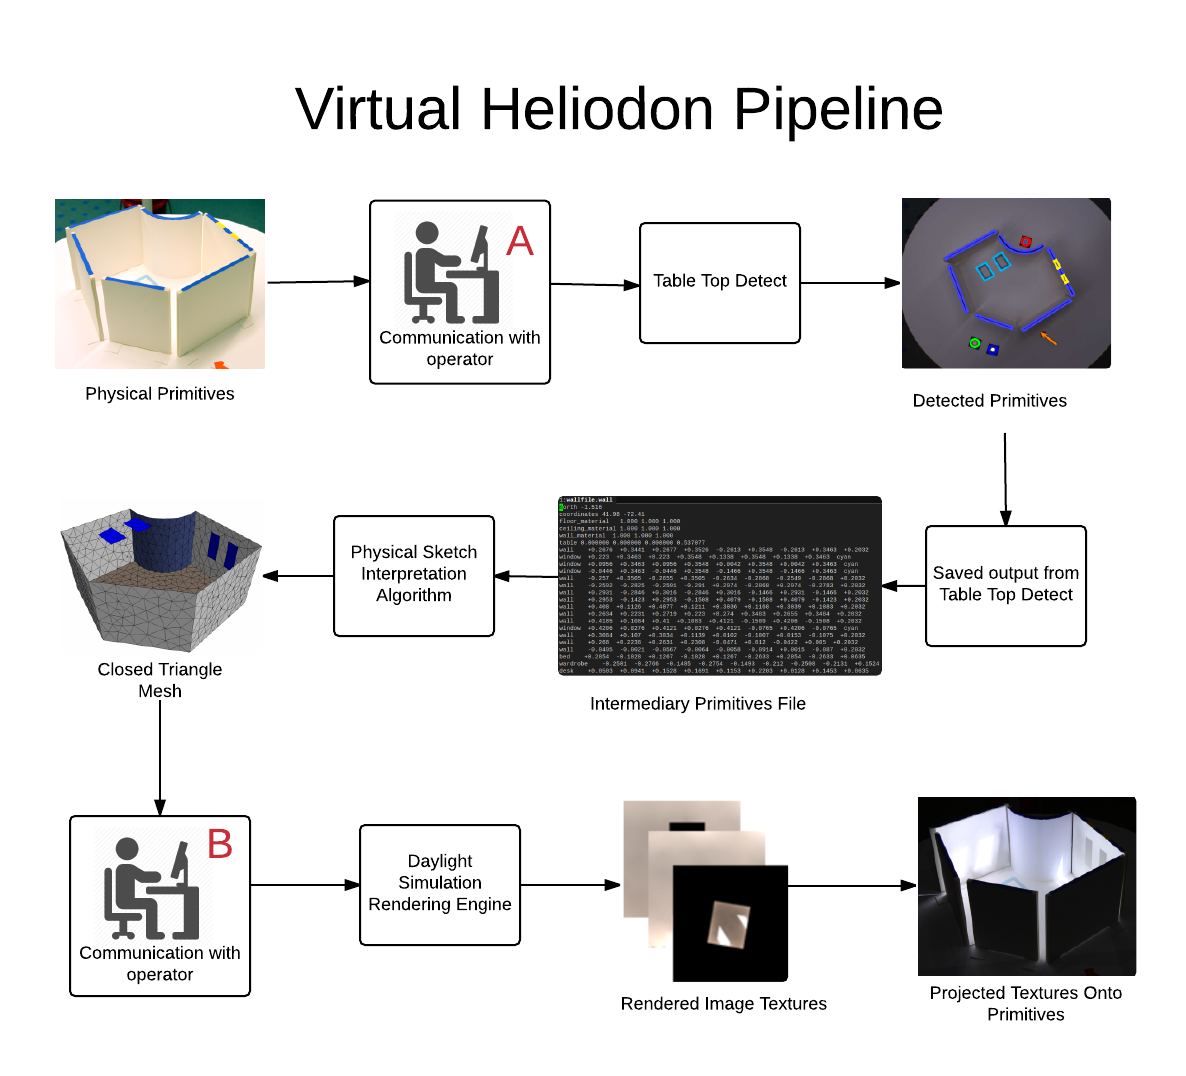
\includegraphics[width=1.0\textwidth]{pipeline_vh}
\caption{Virtual Heliodon's simplified pipeline. A and B are locations in the pipeline that require an experienced operator to perform technical actives on the Virtual Heliodon. }
\label{fig:new_pipeline}
\end{figure}

\paragraph{OASIS Pipeline}
OASIS is an alternative interface to the Virtual Heliodon. 
The system pipeline in Figure-\ref{fig:new_pipeline} illustrates the components involved in OASIS.
In addition, Figure-\ref{fig:new_pipeline} emphasizes all portions of OASIS that I directly contributed to.
To begin, users on OASIS generate 2D sketches consisting of lines that represent wall and windows and objects that represent furniture items.
The physical sketch interpretation algorithm that the Virtual Heliodon uses to generate watertight 3D meshes for simulations require sketches be given as a collection of model primitives. 
Therefore, before being able to invoke the physical sketch interpretation algorithm, OASIS generates the intermediate primitives file.
Model primitives are stored in an intermediate primitives file where each line describes a wall,window, or furniture item in a sketch.
As mentioned previously, in the Virtual Heliodon the intermediate primitives file is created by a simple computer vision algorithm that detects walls, windows, and tokens through colored markers placed on the top of physical primitives.
Since the sketching interface is purely in-software, I can directly create this intermediate primitives file without need of a computer vision algorithm to detect primitives.
Interestingly, OASIS avoids a few limitations of the Virtual Heliodon by bypassing the need to detect physical primitives. 
OASIS can support a wider vocabulary of primitives because it is not bound to the detection of colored tokens.
Additionally, at certain angles parallel wall primitives in close proximity to each other on the Virtual Heliodon could result in the occlusion of primitives in the overhead image. 
Since OASIS is an in-software solution, this problem is avoided as the position of all primitives is always known.
Figure-\ref{fig:new_pipeline}A illustrates where OASIS generates the intermediate primitives file in our system pipeline.
Given the intermediate primitives file the physical sketch interpretation algorithm outputs a closed triangle mesh that the user can view in the \textit{Generate 3D Model} page.
The user can create a daylight simulation request in the \textit{Create Daylighting Simulation} page, given confirmation that a 3D generated model matches the user's intention.
This portion of the system pipeline is illustrated in Figure-\ref{fig:new_pipeline}B.
After the submission of a daylight simulation request, I use the daylight simulation rendering engine to produce texture images.
These texture images capture global illumination from a daylight simulation in a viewpoint independent manner.
On the \textit{Analyze Daylighting} page, I map these texture images onto the 3D mesh to display a daylight rendering of the user's generated model.
Figure-\ref{fig:new_pipeline}C illustrates where texture mapping occurs in the system pipeline.
In brief, our pipeline shows that OASIS is an alternative autonomous interface to the physical sketch interpretation algorithm and daylight rendering engine used in the Virtual Heliodon.

\begin{figure}[h]
\centering
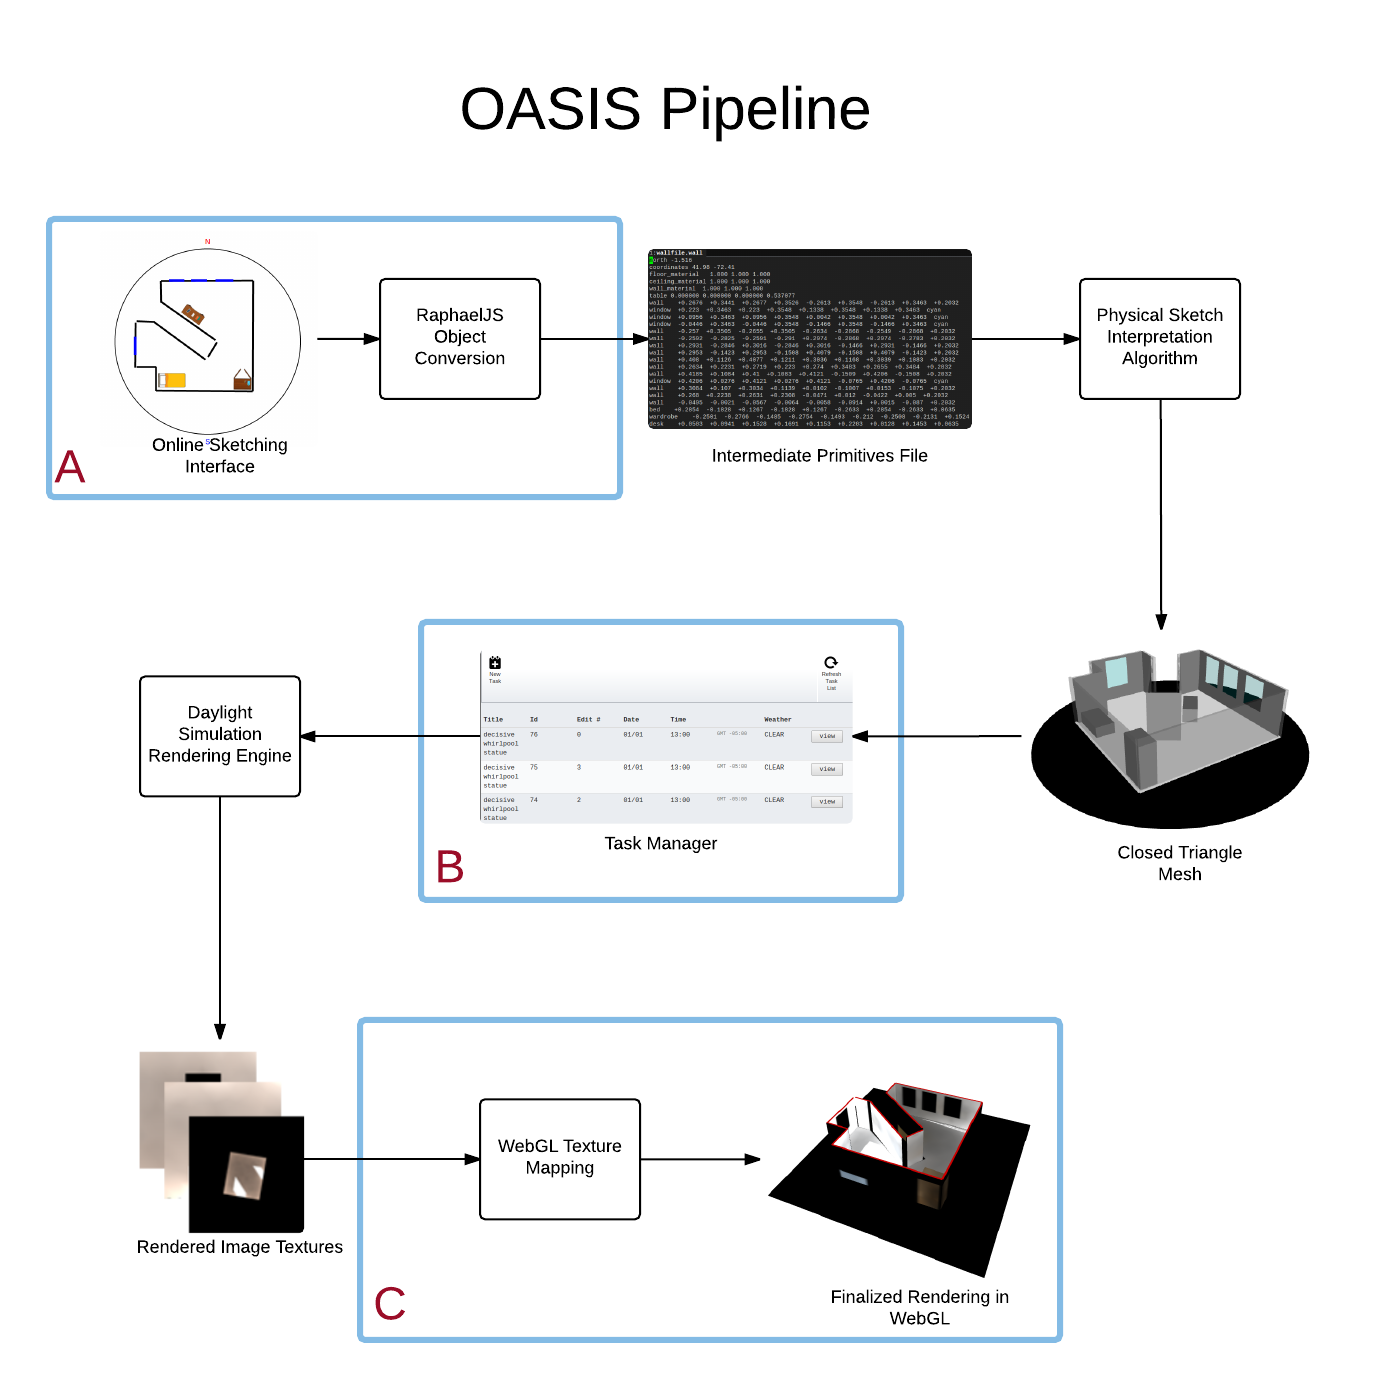
\includegraphics[width=1.0\textwidth]{new_pipeline}
\caption{OASIS pipeline diagram with the author's contributions noted in blue.}
\label{fig:new_pipeline}
\end{figure}

\paragraph{Basic Navigation and Pages}

OASIS consist of six pages that users can navigate between linearly and non-linearly; these pages are illustrated in Figure-\ref{fig:overview}.
Each of these pages, with the exception of the login/register page, are accessible through respective tabs located at the top most portion of the page.
Each respective page, allows users to interact with different portions of our system pipeline.
For beginners it is recommended that pages are followed linearly from step 1 to step 5.
Figure-\ref{fig:overview}A illustrates the first page users encounter when opening our web application.
The \textit{Login/Registration} page is designed to be as minimal as possible to encourage users to register and try out OASIS.
After a successful login or registration, the first page users are directed to is the \textit{Create/Load Model} page.
The \textit{Create/Load Model} page contains a selectable list of users' previously created sketches and the option to create new sketches.
The \textit{Create/Load Model} page is illustrated in Figure-\ref{fig:overview}B.
Assuming users follow the pipeline linearly, users would either load previously created models or start new models.
Either action would result in a redirection to the \textit{Sketch a Room} page, shown in Figure-\ref{fig:overview}C.
The \textit{Sketch a Room} page contains the architectural sketching interface.
After the user is satisfied with their sketch they can proceed to the \textit{Generate 3D Model} page.
Visiting the \textit{Generate 3D Model} page will invoke the generation of an intermediate primitives file; afterward OASIS passes the intermediate primitives file to the physical sketch interpretation algorithm. This creates a 3D watertight triangle mesh object that is displayed on the \textit{Generate 3D Model} page.
Figure-\ref{fig:overview}D illustrates the \textit{Generate 3D Model} page.
Depending on the 3D watertight triangle mesh object created the user can either confirm their intention was met and navigate to the \textit{Create Daylighting Simulation} page or navigate back to the \textit{Sketch a Room} page to make alterations.
On the \textit{Create Daylighting Simulation} page the user can either create new daylight renderings or view previously created renderings, as seen in Figure-\ref{fig:overview}E.
After the creation of a rendering users can then click on the \textit{view} button associated with the rendering of interest.
Clicking the \textit{view} button will redirect users to the \textit{Analyze Simulation} page.
The \textit{Analyze Simulation} page will display a daylight rendering that users can interact with for analysis.
Figure-\ref{fig:overview}F illustrates the \textit{Analyze Simulation} page.
The \textit{Analyze Simulation} page will also host a variety of daylight visualizations that users can toggle between to perform both qualitative and quantitative daylight analysis.
All in all, we hope that OASIS has a small learning curve and allows users to quickly preform daylight analysis with the least cost of effort.

\begin{figure}[h]
\centering
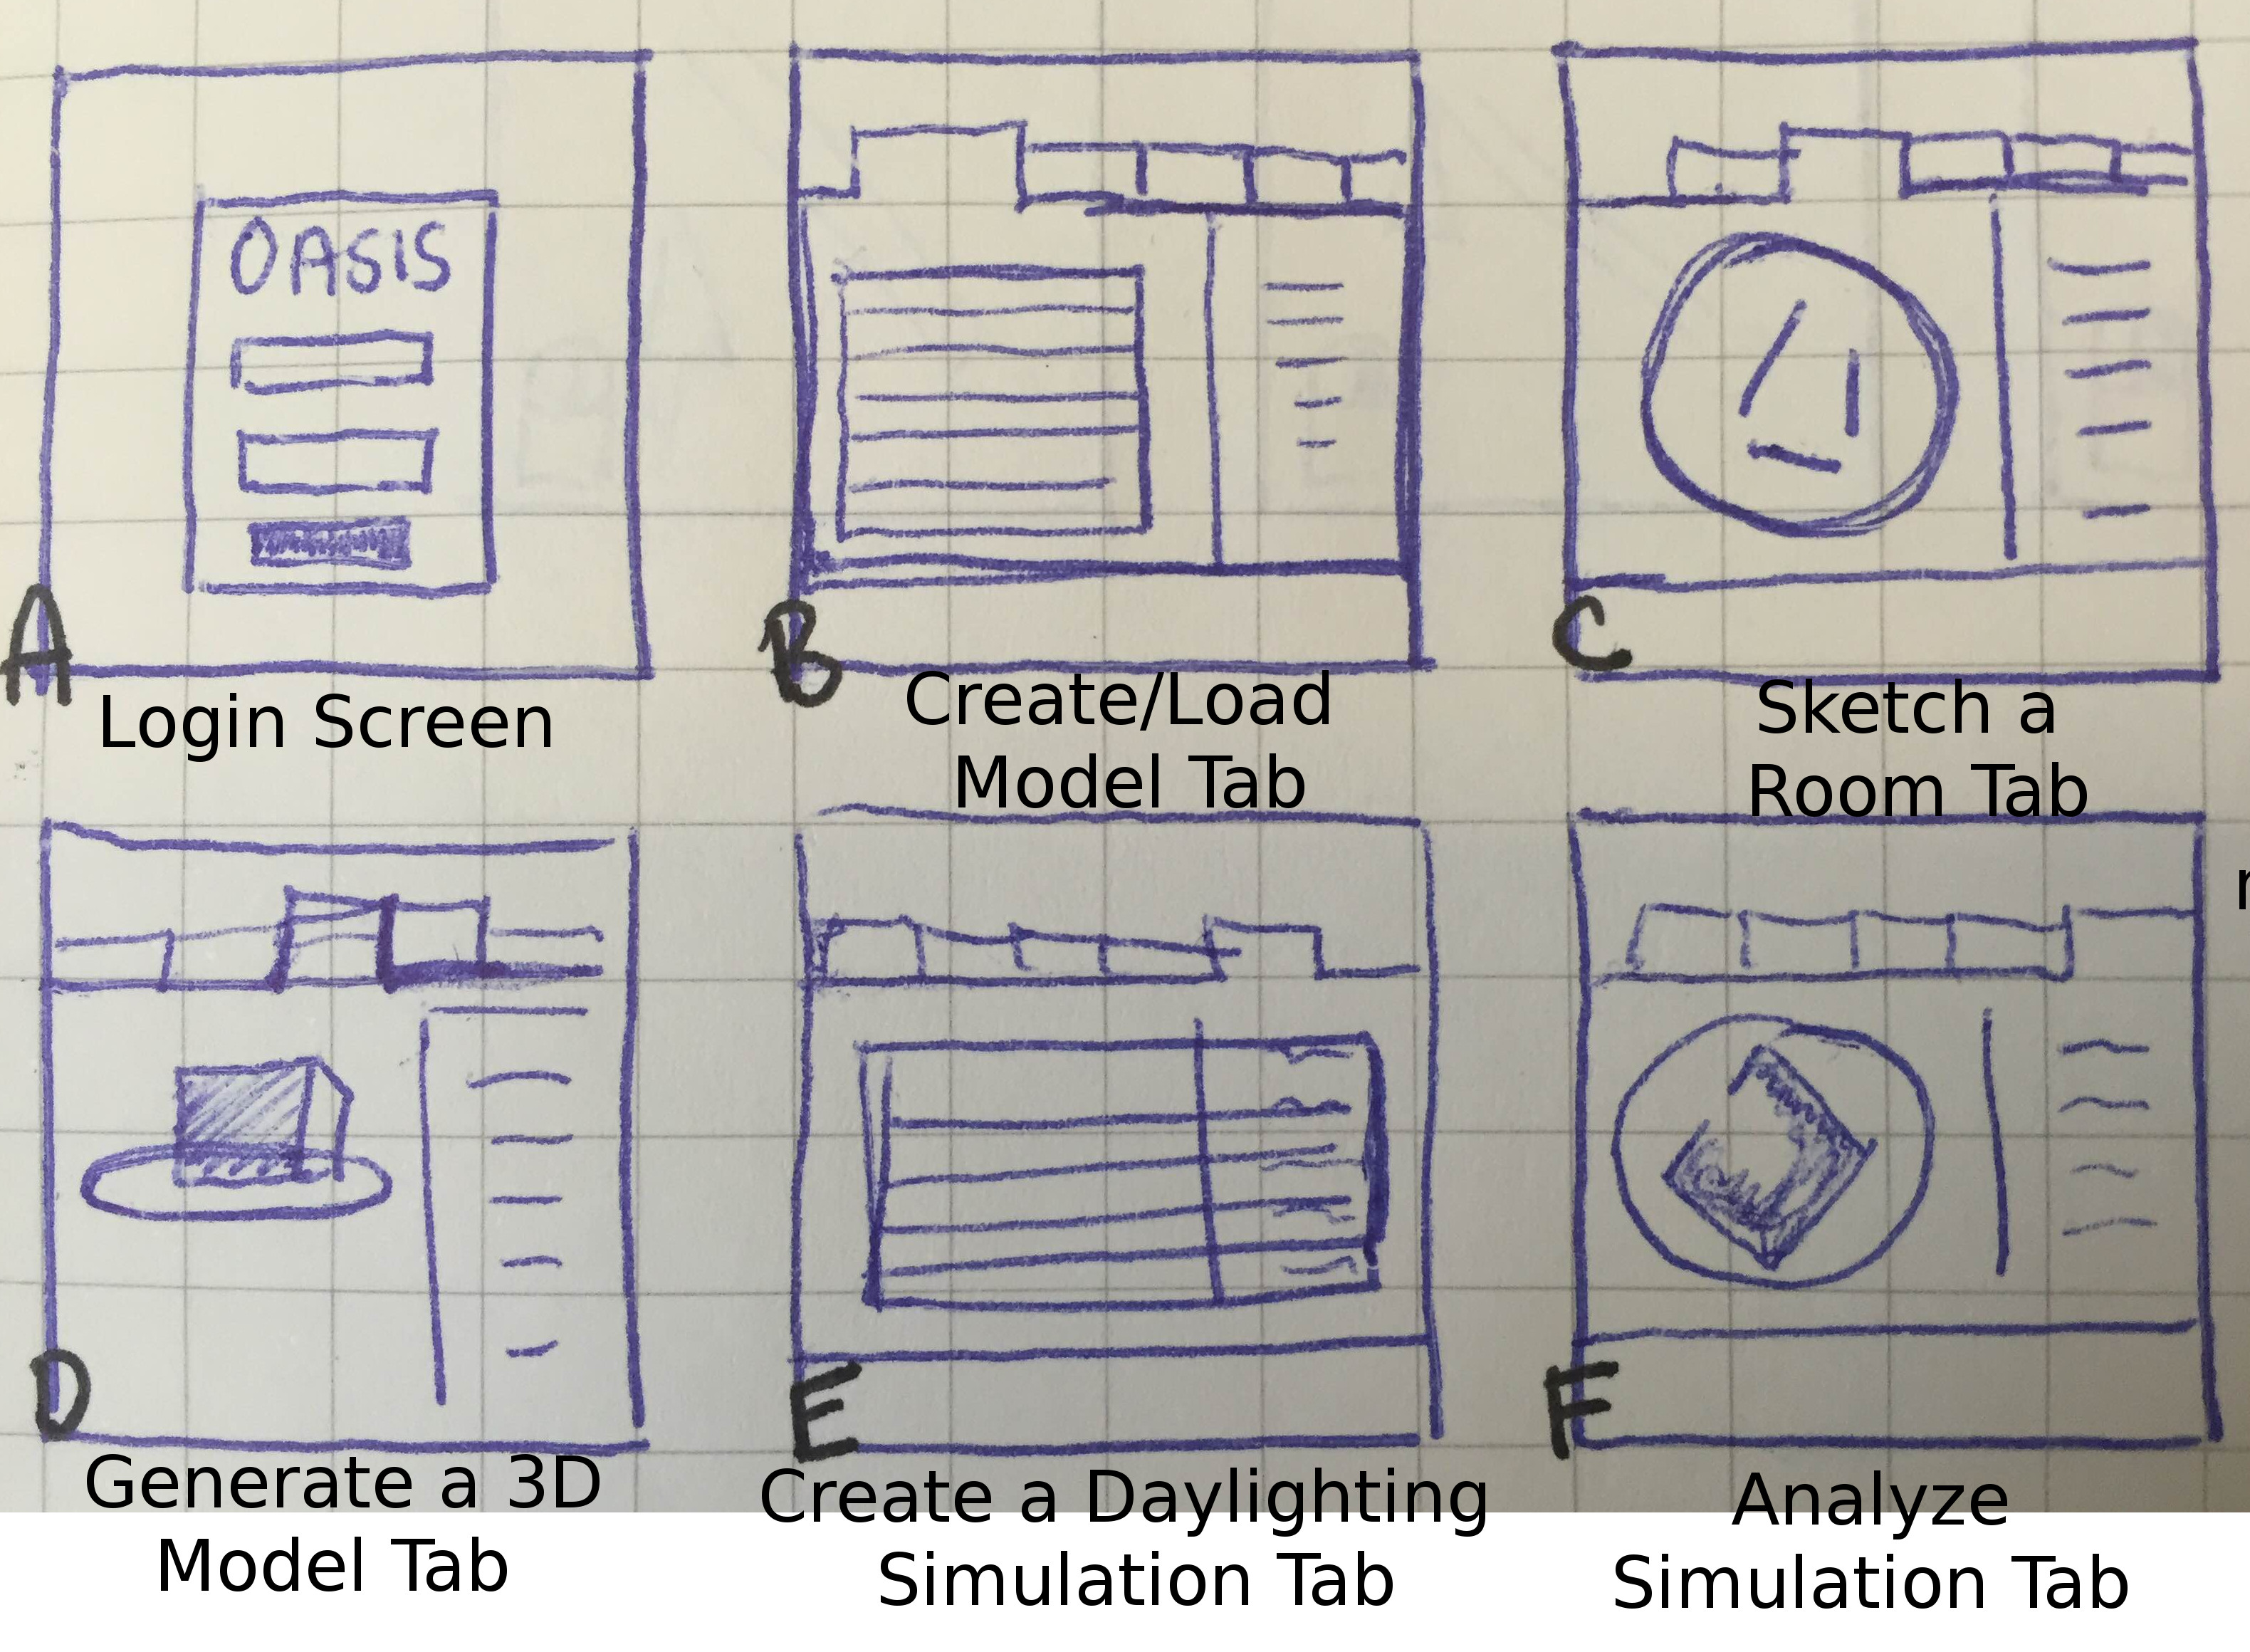
\includegraphics[width=0.8\textwidth]{overview}
\caption{This is an overview of the pages on OASIS.}
\label{fig:overview}
\end{figure}

\paragraph{Importance of UI}\label{ui_importance}
A previous survey discovered that on average 48\% of written code for a given application is made up of user interface implementation\cite{Myers1992}.
The same survey also noticed that 50\% of time spend coding an application is devoted to implementing the user interface\cite{Myers1992}.
User interface design is important to the success and usability of any piece of software.
Bottlenecks in a tool's user interface can result in user frustration and a reduction in users' productivity.
% <Discussion of Current UI?>
As a result OASIS is intended to provide an autonomous easy-to-use interface for interacting with the physical sketch interpretation algorithm and daylight rendering engine.
Notably, we define easy-to-use  as a general term that refers to the lack of formal training required to use a tool.
As discussed previously, the interface in the Virtual Heliodon requires an experienced operator at all times.
It is important to note that there has been attempts to give users control over the Virtual Heliodon including programming a remote clicker to trigger the \textit{table top detection} process.
However, there is currently no user interface for choosing visualizations to display and define the parameters required by those visualizations.
The Virtual Heliodon, just like OASIS, aims to be an easy-to-use interface for not only the design of architectural spaces but also the generation of helpful visualizations.
Requiring an operator with programming experience and background knowledge on the Virtual Heliodon may hinder users' creative iterative design process.
% < Closing statement of UI>
By and large, the user interface can make or break an application and as a result we stress the importance of interfaces that are both autonomous and easy-to-use.

\section{Sketching Interface Design}

\subsection{Sketching Walls and Windows}
% Why is sketching walls/win important
The boundaries that define an architectural space are composed of walls and other dividing objects.
The  boundaries of an architectural space must be well defined, in order to produce a 3D watertight triangle mesh.
The physical sketch interpretation algorithm differentiates the interior and exterior of a sketch in the process of generating a 3D watertight triangle mesh.
Consequently, the physical sketch interpretation algorithm requires walls to perform this differentiation\cite{cutler2010interpreting}.
The interface that allows users to define where walls in windows are placed in a sketch is important to the generation of 3D watertight triangle meshes and the overall usability of OASIS.\\
 
% Discussion about what we do
OASIS mimics physical drawing via a click-draw-release procedure.
The click-draw-release procedure is illustrated in Figure-\ref{fig:wall_win}.
In order to draw walls users must first toggle the \textit{wall drawing} mode on OASIS;
Toggling the \textit{wall drawing} mode is done by clicking on the \textit{wall} button located at the top of the \textit{Sketch a Room} page, as illustrated in Figure-\ref{fig:wall_win}A.
% Checkpoint
Then, as Figure-\ref{fig:wall_win}B and C illustrate, by holding the left mouse button and dragging anywhere on the canvas the user is shown a preview of where a wall will be drawn.
By releasing the left mouse button, the wall preview will be replaced by a drawn line, representing a wall, as Figure-\ref{fig:wall_win}D depicts.
Once a wall is drawn further editing is not allowed.
To keep with the spirit of sketching, windows are also placed into a sketch by being drawn similarly to walls, as shown in Figure-\ref{fig:wall_win}E through G.
However, unlike walls, windows need to be associated with a wall.
As a result a window needs to be drawn on or near a wall.
In the interest of the user, windows do not need to be drawn exactly on walls.
A window when drawn near a wall sharing a similar angle will automatically target and snap onto that wall, as illustrated in Figure-\ref{fig:wall_win}H.
This snapping feature makes drawing windows less reliant on users' precision with their input device, but rather focuses on users' intention. \\

% Discussion about alternatives(old method)
An alternative interface that was implemented but not used, allows users to create walls and windows via a drag-and-drop procedure;
The drag-and-drop procedure is illustrated in figure-\ref{fig:oldvh}D through F.
Users could then further manipulate walls and windows by both rotating and scaling them through the use of FreeTransform handles. 
FreeTransform handles are three white circular handles that are overlaid onto walls and windows.
One circle appears at the center and another circle is placed some distance away from the wall or window, as illustrated in Figure-\ref{fig:oldvh}F.
The circular handle in the center can be used to translate the primitive to anywhere on the canvas.
The circular handle off the side of the primitive is used to both scale and rotate the primitive to a desired length and angle.
Moreover, Figure-\ref{fig:oldvh} illustrates the parallels between how users place walls  into a scene in both the Virtual Heliodon and via the drag-and-drop procedure.
Both Figure-\ref{fig:oldvh}A and D illustrate how users have to select a primitive from a collection of primitives in both the Virtual Heliodon and via the drag-and-drop procedure.
Figure-\ref{fig:oldvh}B and E show how users have to place selected primitives on a surface, such as the physical table top or the online interface's canvas.
Figure-\ref{fig:oldvh}C and F demonstrate how users adjust either physical primates through physical interaction or the manipulation of FreeTransform handles.
However, despite mimicking how primitives were placed in the Virtual Heliodon, our eventual goal with OASIS is to pursue the most intuitive interface for drawing walls and windows.
The  drag-and-drop procedure focused on mimicking user interaction on the tangible user interface.
Overall, further testing, such as A/B testing, would be required before any conclusions can be drawn as to which interface is more intuitive.\\

\begin{figure}[h]
\centering
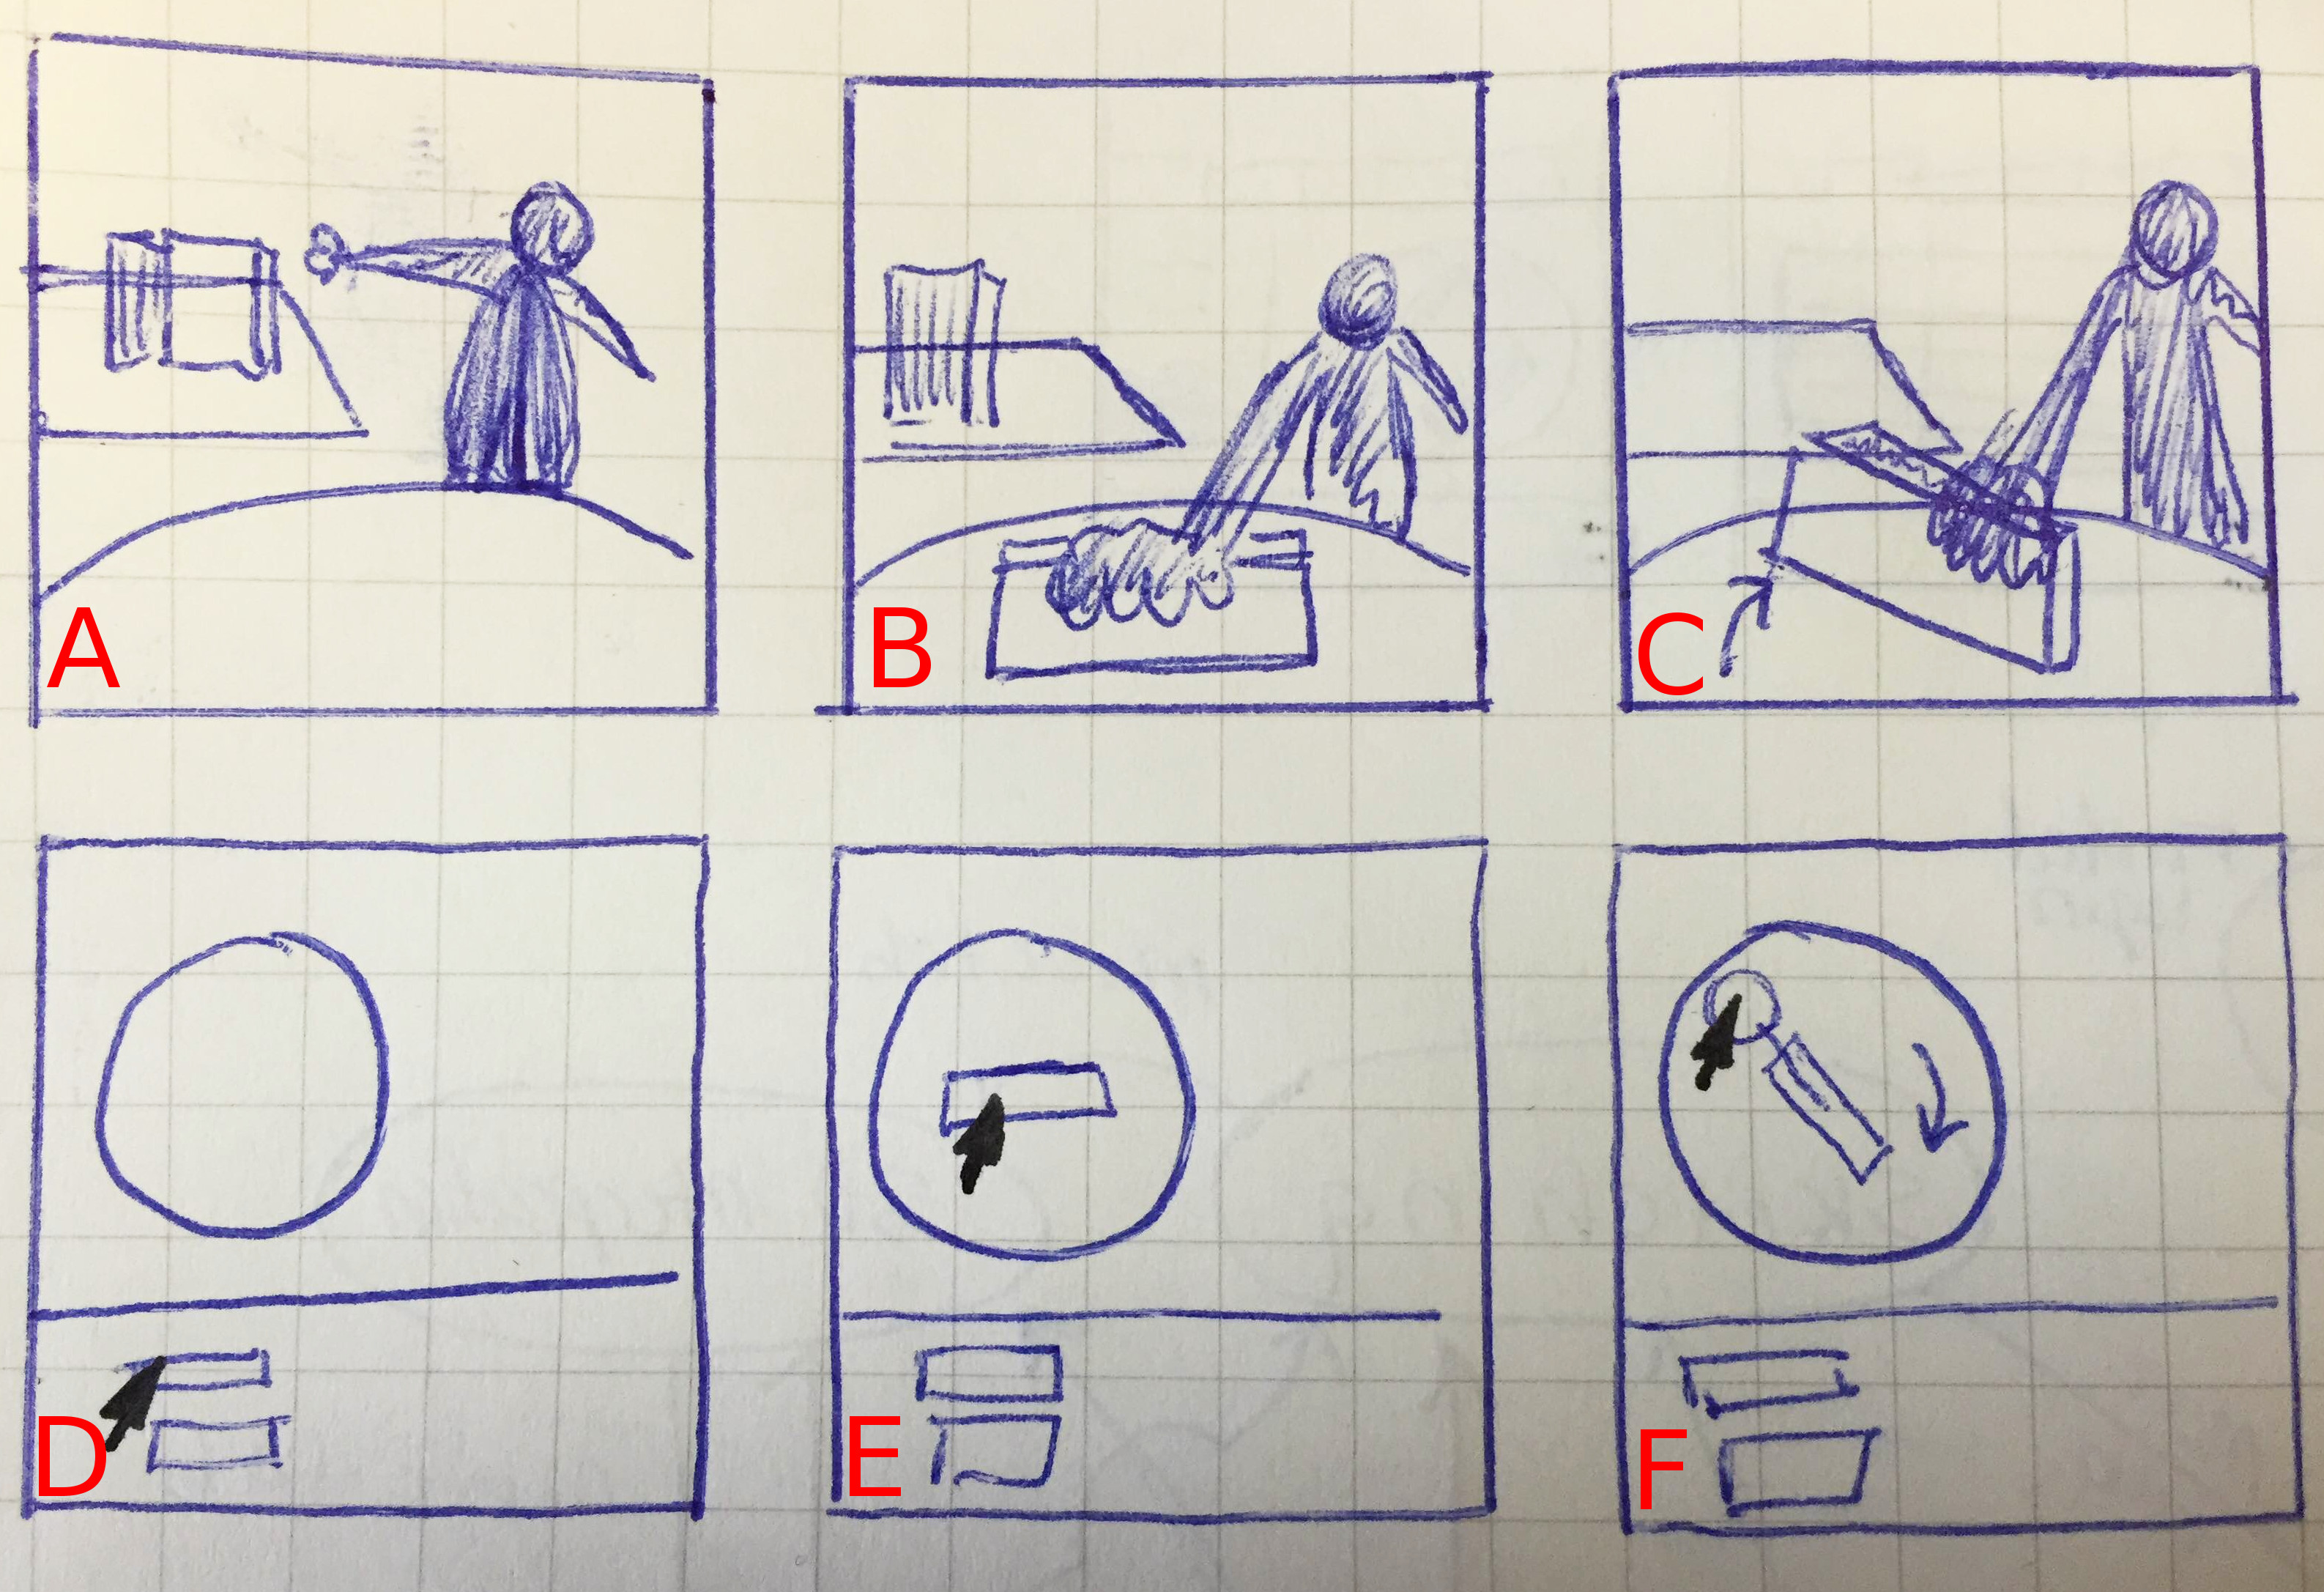
\includegraphics[width=0.8\textwidth]{oldvh}
\caption{
Similarities between the drag-and-drop procedure and the Virtual Heliodon's Tangible User Interface. 
% A) Users select a physical primitive from a collection of primitives. 
% B) Users place primitive on the table top. 
% C) Users adjust the primitive as desired. 
% D) Users select a primitive from a tray on the bottom of the interface. 
% E) Users drag that item onto the table. 
% F) Users use FreeTransform handles to scale and rotate the primitive as desired.
}
\label{fig:oldvh}
\end{figure}

\begin{figure}[h]
\centering
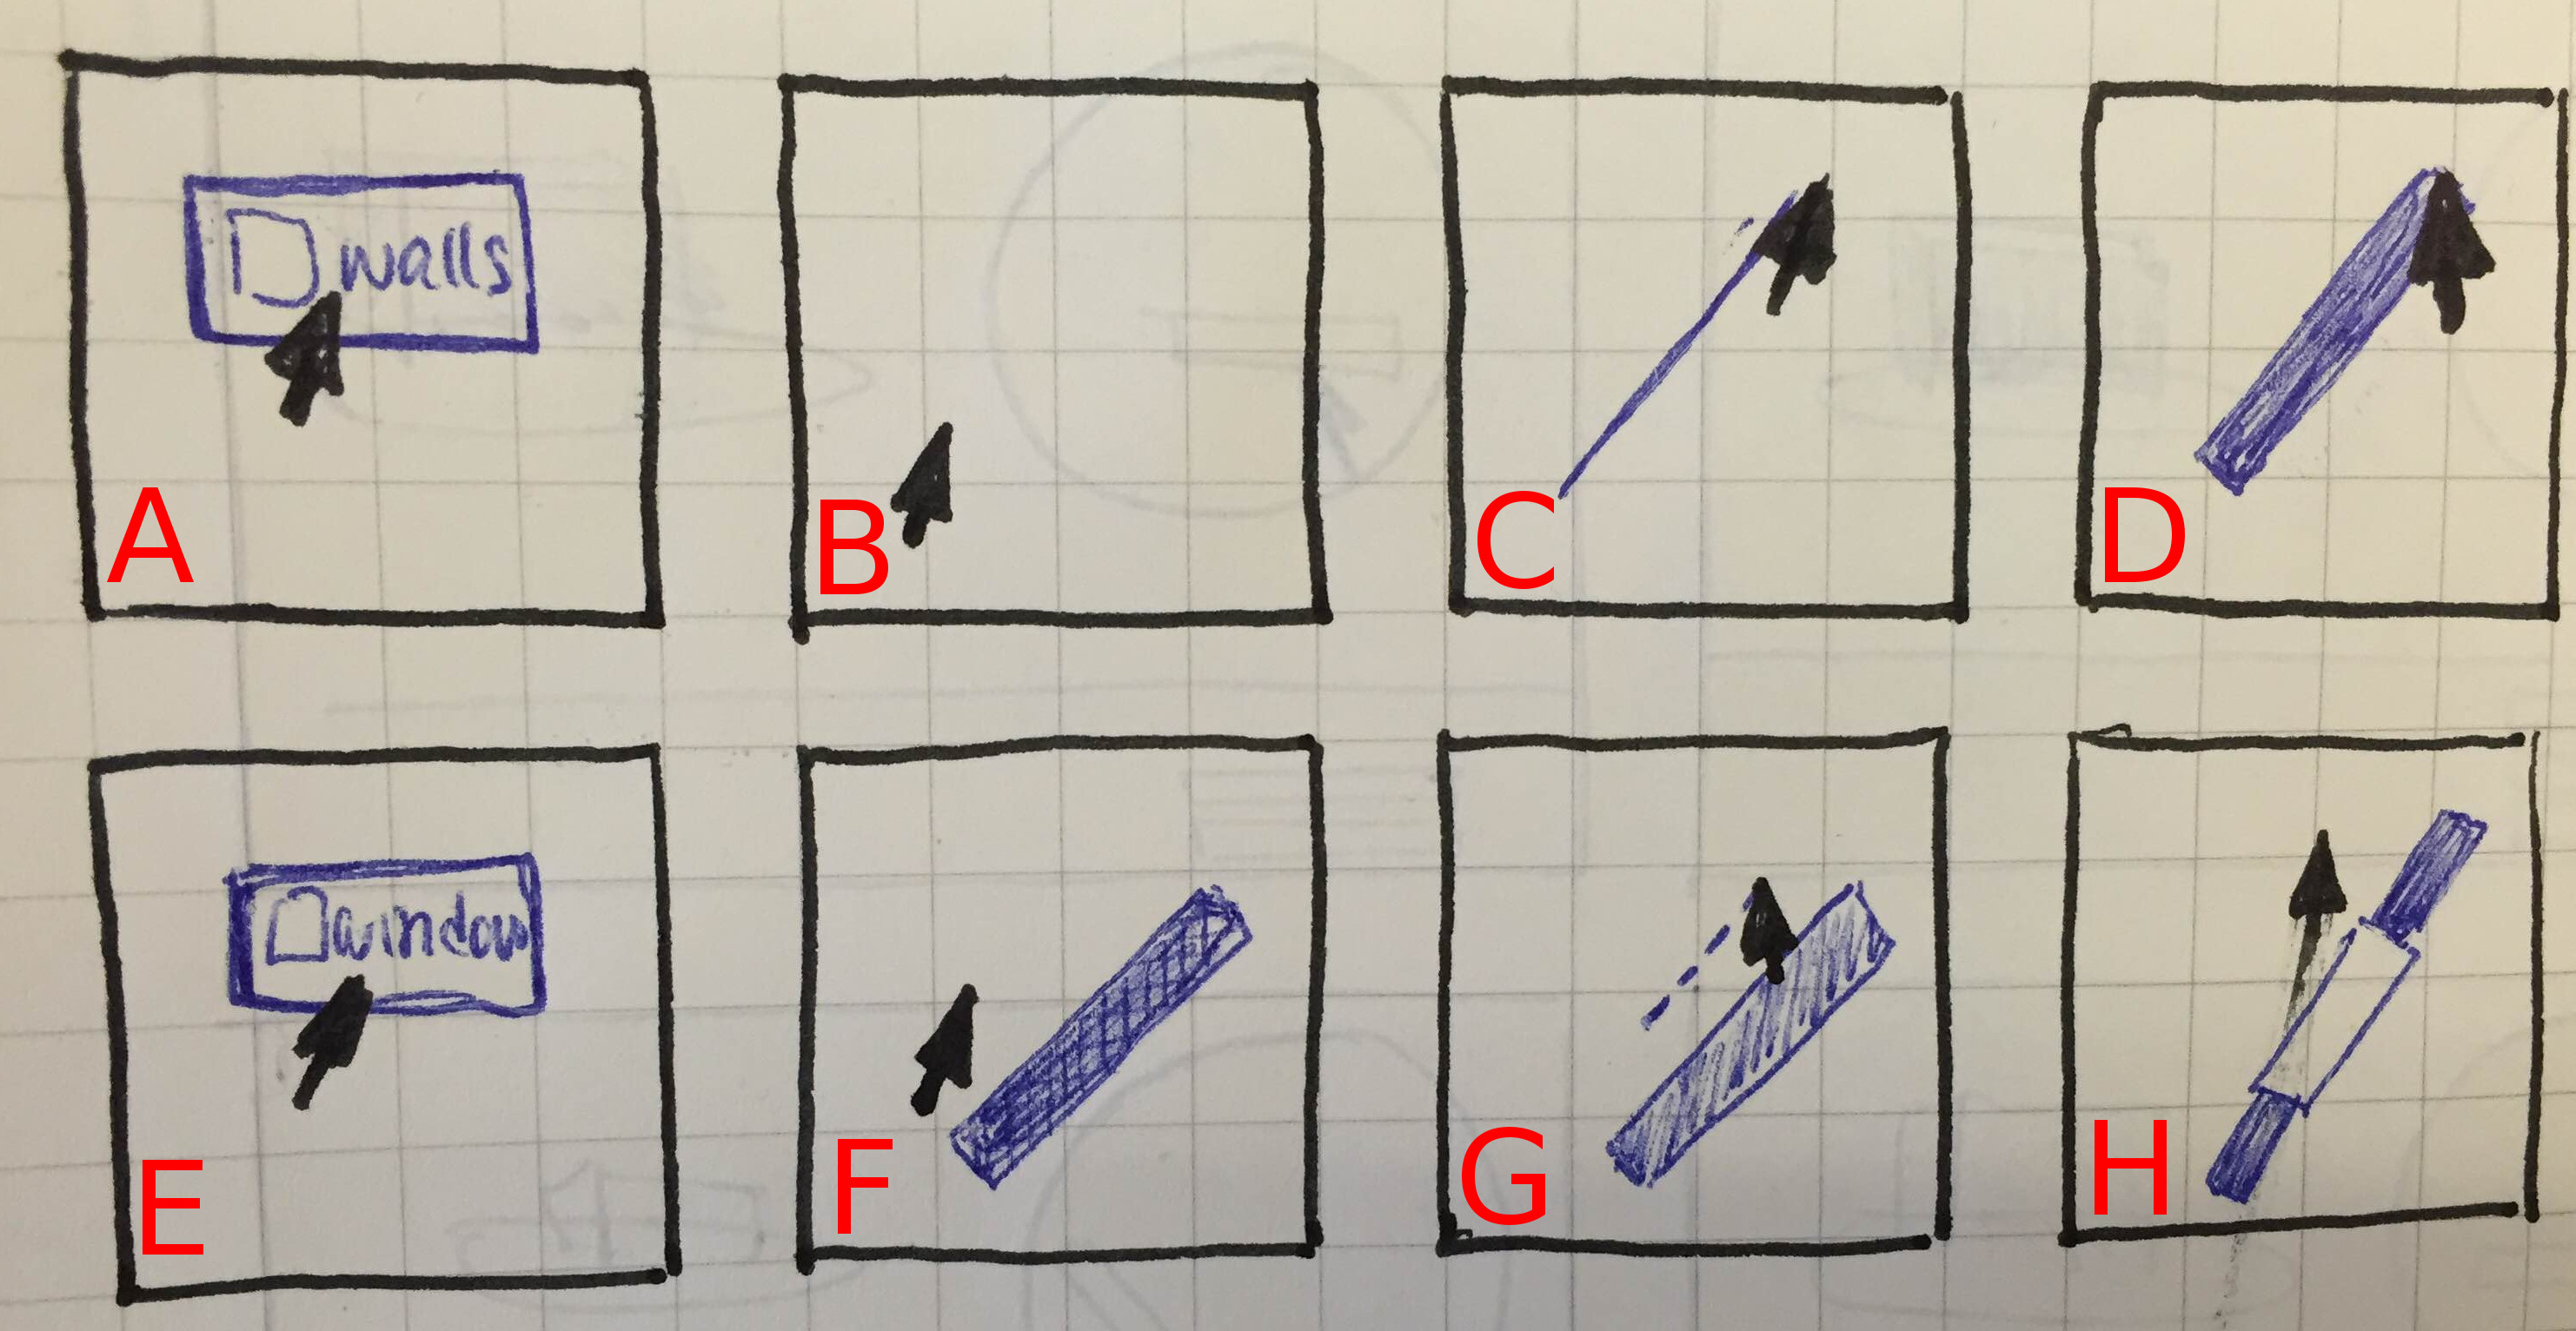
\includegraphics[width=0.8\textwidth]{wall_win}
\caption{How to create walls and windows via the click-draw-release procedure.}
\label{fig:wall_win}
\end{figure}

% Discussion about Eric's work
Additionally, OASIS is currently undergoing the investigation of a new sketching interface that would allow users to draw free form lines, shapes, and letters.
Using this new sketching interface users could traditionally draw walls and windows to define architectural sketches on OASIS.
User's drawing accuracy can vary dramatically depending on the input devices users are drawing with; common input devices includes computer mouses, touch screens, and pen-based drawing tablets.
This new interface is investigating how to correct users' sketches to  generate the intermediate primitives file required to create  3D closed meshes for simulations.
Extensive A/B testing between these three methods of sketching walls and windows  would be required to to decide which interface is most intuitive to users.

\paragraph{Furniture Placement}

Another difference between OASIS and the Virtual Heliodon is the support of furniture items.
Walls and windows are not the only elements that affect daylighting;
furniture can also occlude, diffuse, and reflect daylight.
Moreover, daylight distribution is scale invariant and as a result the Virtual Heliodon did not concern itself much with communicating to users a sense of scale.
We currently support statically sized furniture items in OASIS, such as beds, desks, and wardrobes.
These furniture items are used to indirectly communicate a sense of scale to users.
Since furniture items cannot be made larger or smaller, users are forced to sketch architectural spaces in respect to the size of furniture items.
Furthermore unlike walls and windows, furniture items are placed into the canvas by first clicking a furniture item button; these buttons are located on the top of the \textit{Sketch a Room} page.
After choosing a furniture item, OASIS will place the item at the center of the canvas.
Furniture items use the same drag-and-drop procedure as mentioned previously in Figure-\ref{fig:oldvh}.
Users can manipulate furniture items via both translations and rotations. 
Furniture items can be rotated along their center axis via FreeTransform handles attached to the furniture item.
Furniture items can also be translated by clicking and dragging on the item itself.
Item manipulation via drag-and-drop procedures are a common UI mechanism. 
Users will be familiar with these mechanisms if they have had experience using either photo editing software or slide-based presentation tools such as Microsoft PowerPoint\cite{todo}.

% Discussion about future work on sketched furniture items + Dynamic scale??
Additionally, OASIS is currently undergoing the investigation of a new sketching interface that would allow users to draw free form lines, shapes, and letters for not only wall and window placement but also furniture placement.
This interface would allow users to freely draw symbols, that represent furniture items, to determine the position and angle a furniture item will be placed into the canvas.
Interpreting symbols is non-trivial and more research is required before A/B testing can be conducted to determine the advantages of freely drawing furniture items.


\paragraph{Removal of Elements}
OASIS also supports the removal of walls, windows, and furniture items.
Since users cannot reposition their drawn walls and windows after their initial placement, the ability to remove and redraw a wall or window is essential.
The removal of all sketch based elements and furniture is done via a click-to-remove process.
To remove items users must first click on the remove button as illustrated in Figure-\ref{fig:remove}A, secondly users must mouse over the item to be removed as shown in Figure-\ref{fig:remove}B.
Items to be removed upon the left mouse button click are highlighted in red as shown in Figure-\ref{fig:remove}C.
No items are removed from the canvas until the user's left mouse button clicks on a selected item.
An alternative removal mechanism would allowed users to drag walls and windows and ``drop'' elements off the canvas. 
This alternative removal mechanism is intended to mimic the Virtual Heliodon's tangible user interface.
While, OASIS does not support this drag-to-remove procedure,  implementing and A/B testing against this procedure would help us understand which removal procedure users find the most intuitive.

% Include figure
\begin{figure}[h]
\centering
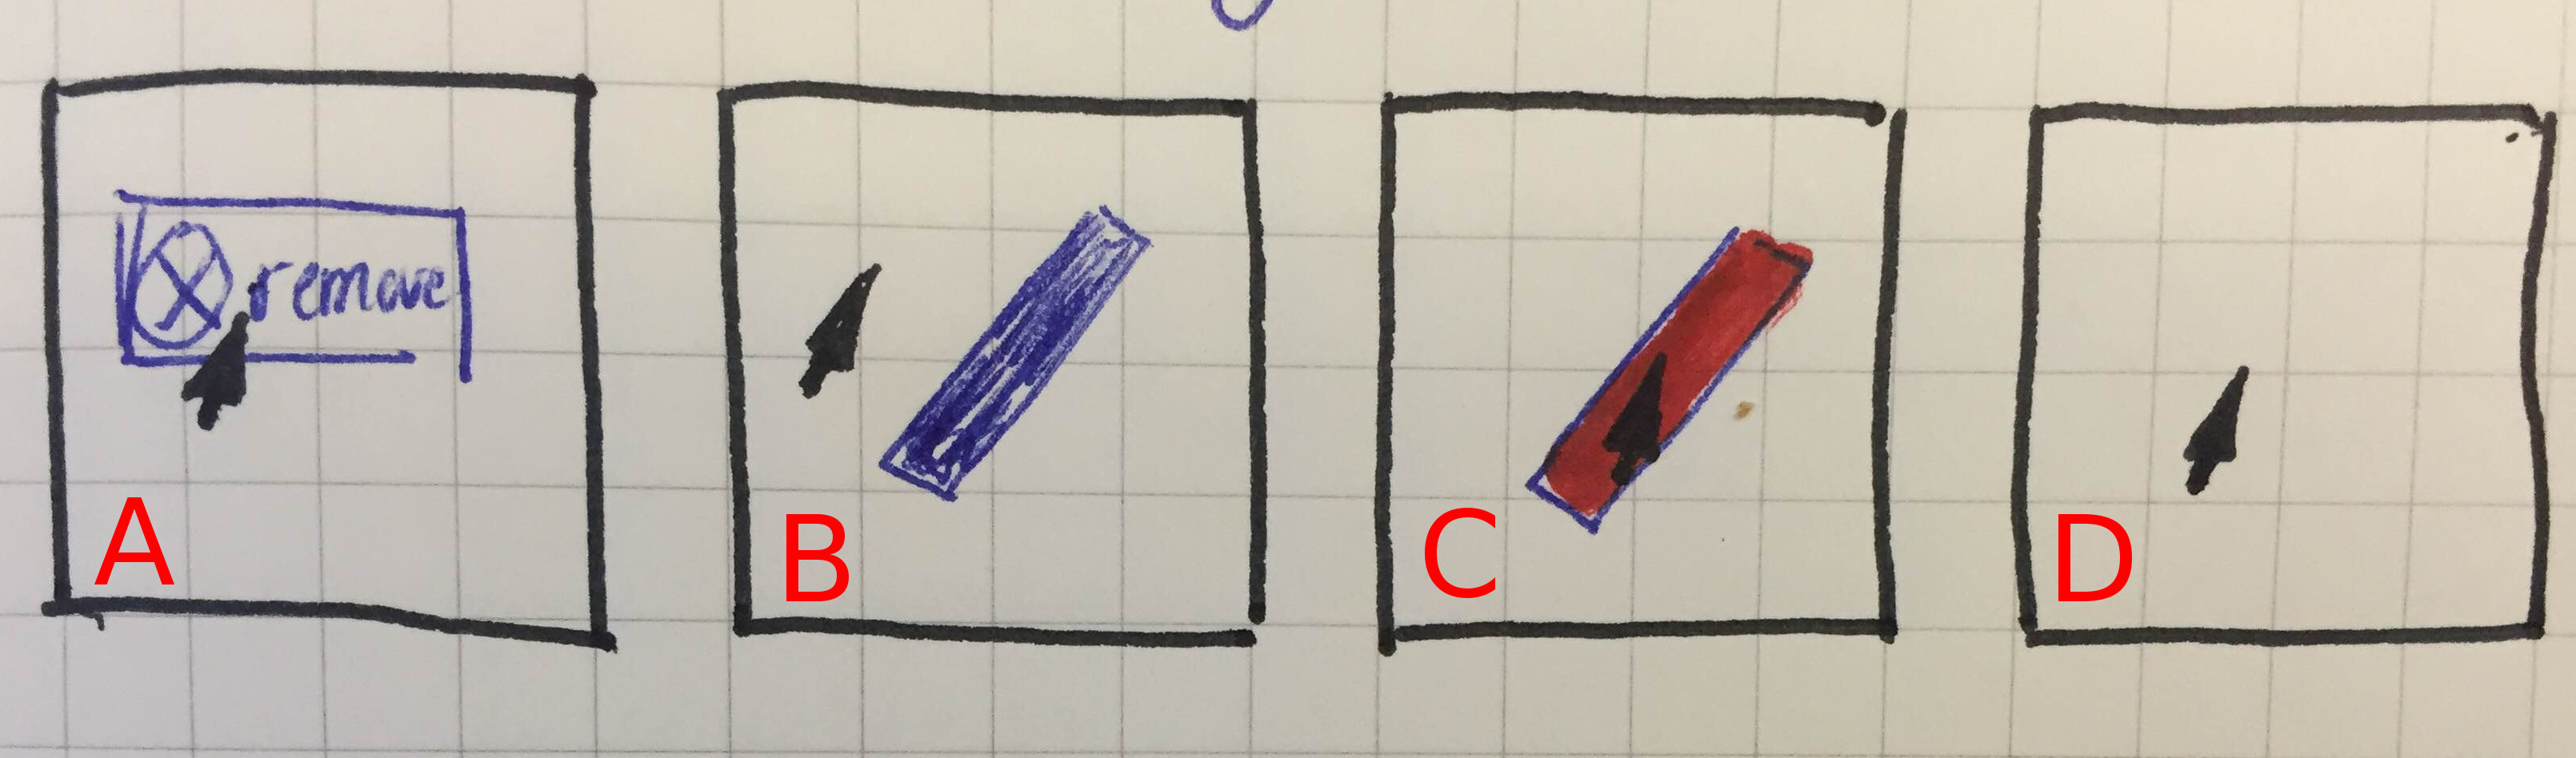
\includegraphics[width=0.8\textwidth]{remove}
\caption{How to remove an item from the canvas via the click-to-remove procedure. 
% A) First users must select the remove button located on the ribbon. 
% B) Second the user must move mouse over the time to be deleted. 
% C) Item to be deleted upon left mouse click is highlighted red. 
% D) If the red highlighted item is the correct item to be removed click the left mouse button. 
}
\label{fig:remove}
\end{figure}

\paragraph{Cardinal Orientation}
% Why is orientation important
The cardinal orientation a of a window has significant impact on daylight distribution in an architectural space.
In OASIS and all daylight analysis tools require that users define cardinal orientation in a architectural space.
Notably, the cardinal orientation of user sketches needs to be defined in order to simulate direct lighting.
% How do we implement it? 
In order to define cardinal orientation users must first click on the orientation button, located in the \textit{Sketch a Room} page's ribbon depicted in Figure-\ref{fig:geoloc}A.
Then users can click and drag anywhere on the canvas to define cardinal orientation.
Specifically, holding the left mouse button on canvas will move the North and South labels around the circumference of the canvas to define the cardinal orientation of the sketch, as shown in Figure-\ref{fig:geoloc}B through D.
% Alternatives
Furthermore, the Virtual Heliodon allows the user to place a north arrow token onto the tabletop to define the cardinal orientation of a physical sketch.
An analogous procedure would require users sketch an arrow on OASIS in order to define the cardinal orientation of their sketches.
Other options include manually typing the model's degree offset from the north arrow; This procedural method of defining the cardinal orientation is common in other daylight software.
Testing would be required to conclude which method of defining cardinal orientation is most intuitive to users.

\begin{figure}[h]
\centering
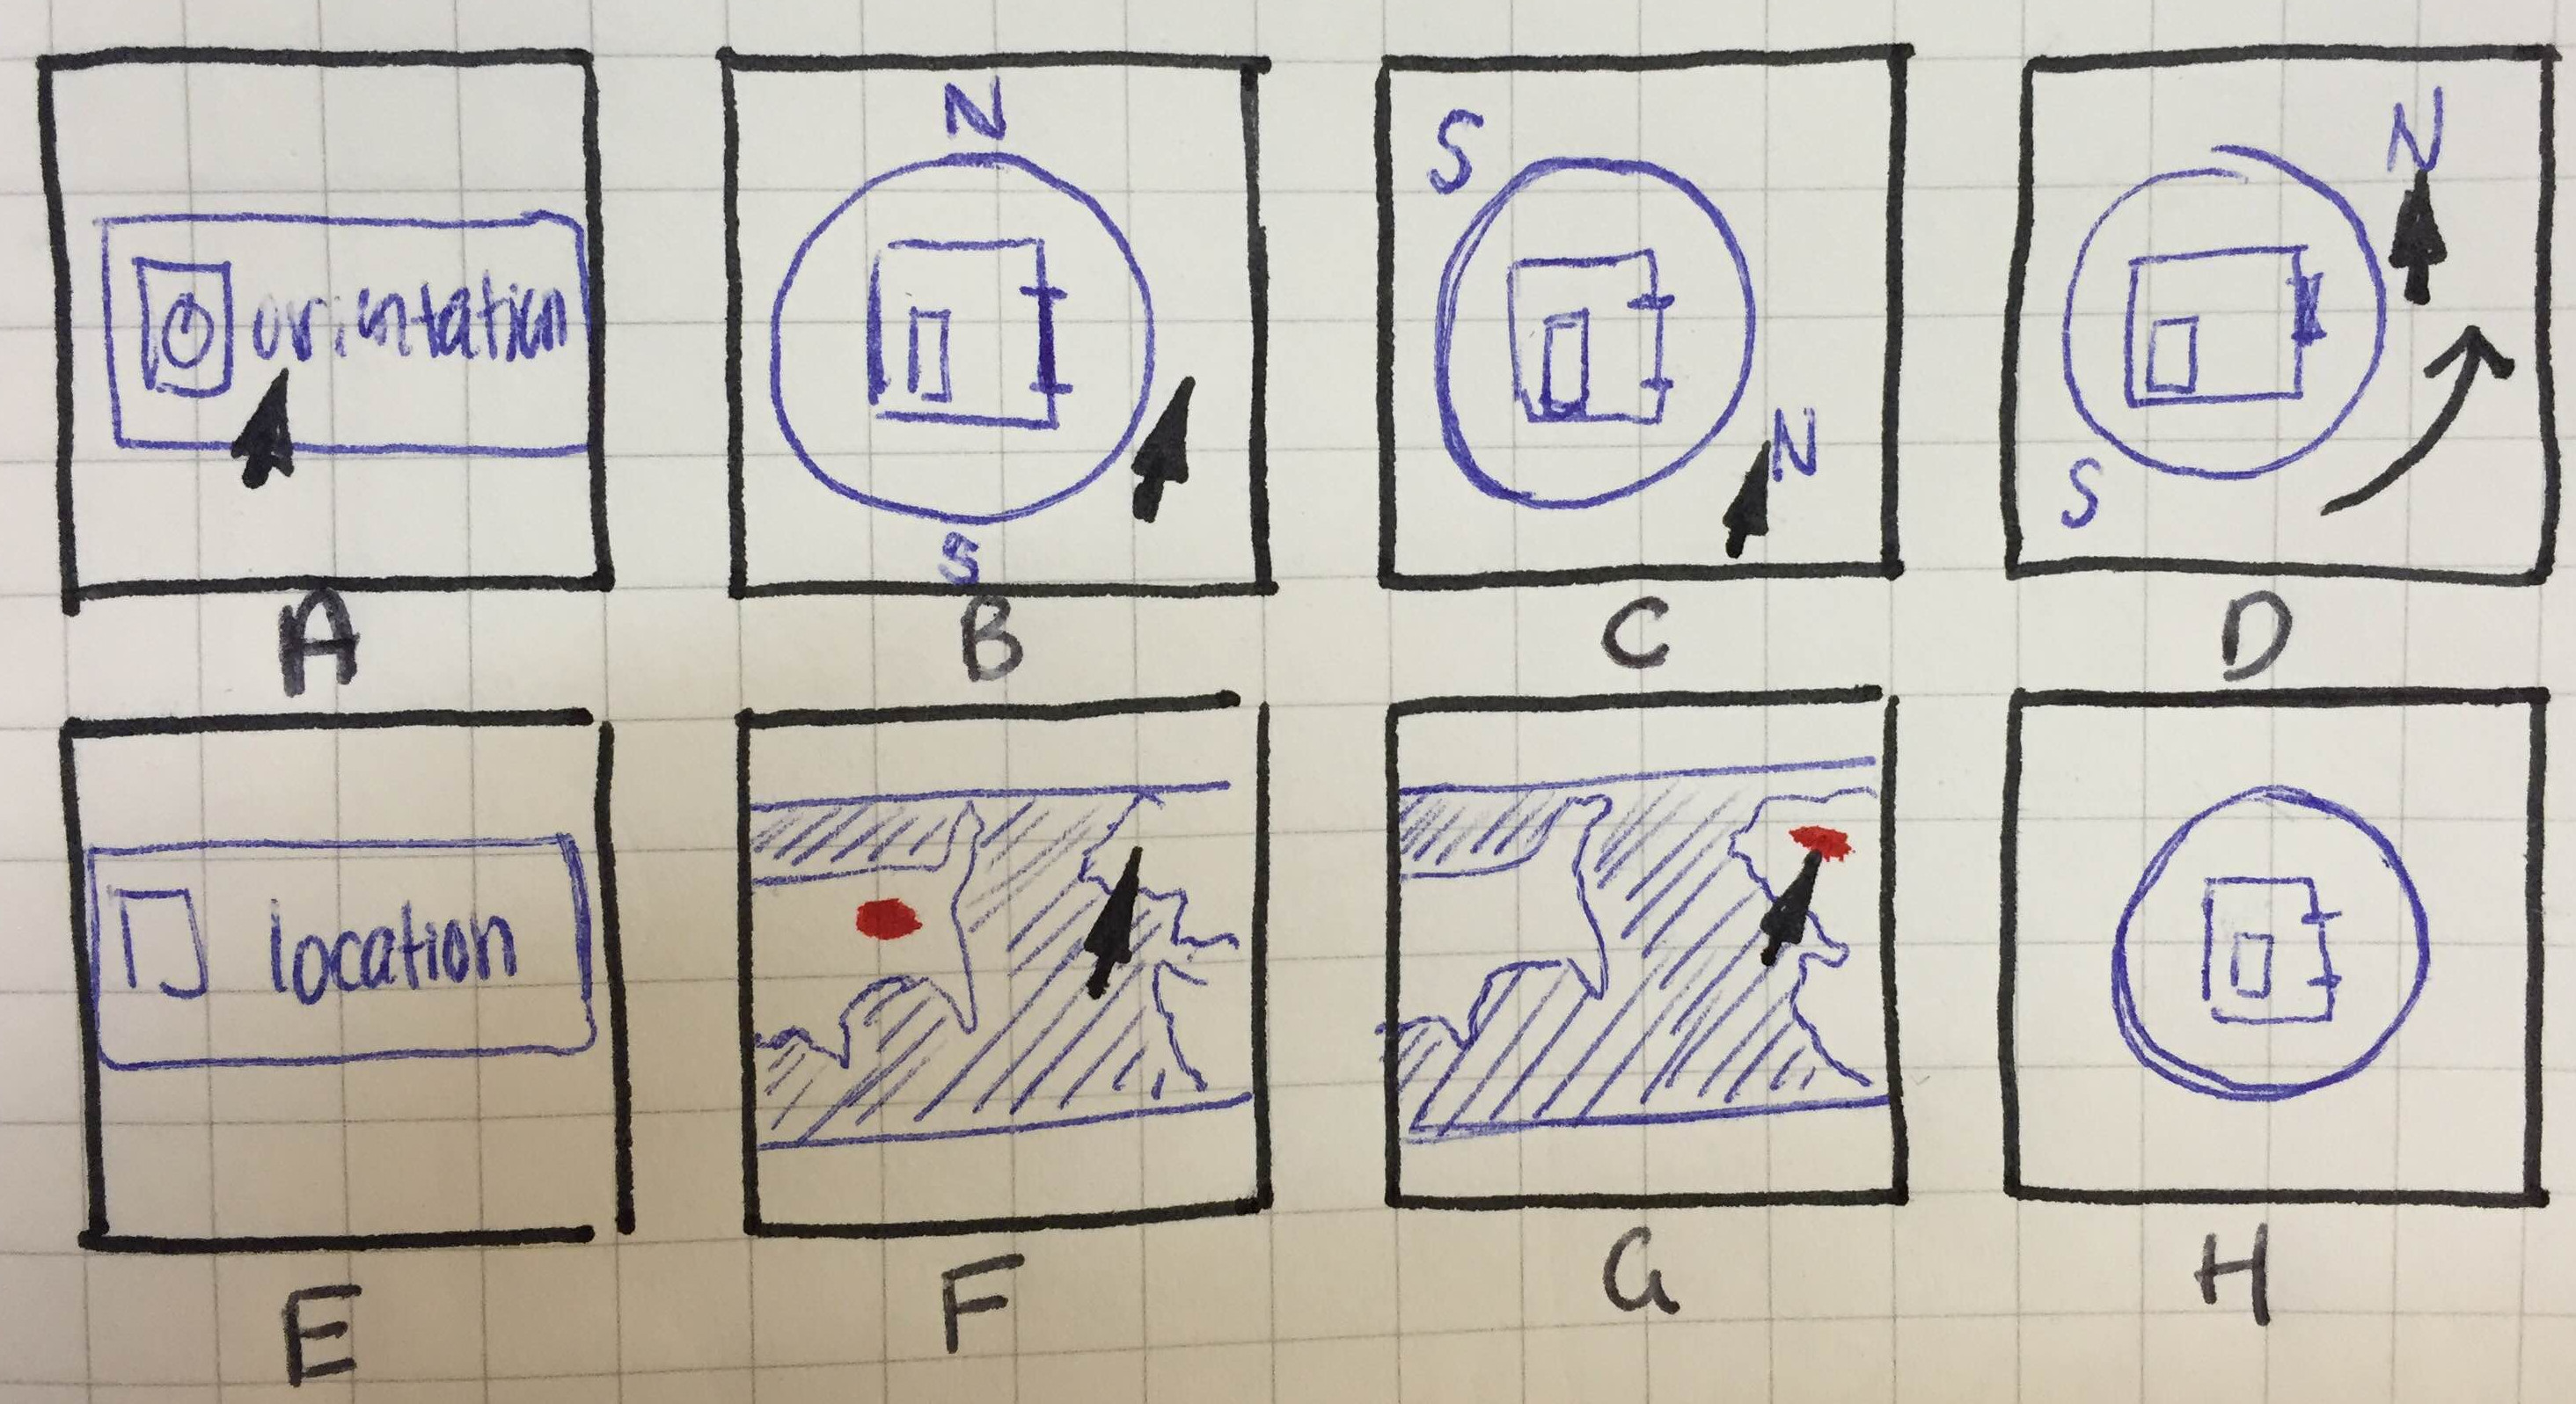
\includegraphics[width=0.8\textwidth]{geoloc}
\caption{
How to set the cardinal orientation and geographical location of a sketch.}
\label{fig:geoloc}
\end{figure}

\paragraph{Geographical Positioning}
Daylight distribution is  not only dependent on an architectural space's cardinal orientation, but also from its geographic location.
South facing windows in the northern hemisphere experience direct sunlight for most of the day, however north facing windows do not.
In the southern hemisphere, the opposite is true; North facing windows experience direct sunlight and south facing windows do not.
Additionally, the sun's highest point in the sky varies from buildings located in the tropics and buildings located outside them.
For these reasons it is important that in OASIS we provide users a way to define a sketche's geographical location.
To define a geographical location users must click on the location button next to the orientation button depicted in Figure-\ref{fig:geoloc}E.
Clicking the location button will bring up a map projection where users can select their model's geographical location by clicking anywhere on the map, as shown in Figure-\ref{fig:geoloc}F and G.
Once the user has selected a location, a red marker is placed on that location and the map  disappears revealing the sketching interface, as depicted in Figure-\ref{fig:geoloc}H.
Users do not need the exact latitude and longitude values because we intend OASIS to be an early design tool. 
Furthermore, daylighting varies significantly depending on what hemisphere a model is located. Daylighting also varies depending on a model's location relative to the equator.
Inaccurately selecting a geographical position off by an entire state or even country will not vary daylighting results much.
Figure-\ref{fig:geoloc} illustrates how a sketch's cardinal orientation and geographical location are defined.
The Virtual Heliodon offers no analogous interface to define geographic location of sketches. 
All sketches in the Virtual Heliodon are set to Troy, NY.
Most daylight analysis software allows users choice from a variety of major cities to define a model's geographic location;
others allow users the ability to input exact geographic coordinates.
Again, testing would be required before any conclusions can be drawn about which method is most intuitive to users for defining the geographic location of models.

\section{3D model viewer}

\paragraph{Sketch Interpretation Viewer}
The sketch interpretation viewer is located on the \textit{Generate 3D Model Page}. This is a simple viewer that displays the 3D watertight mesh created from users' architectural sketches. Users can zoom, rotate, and pan on this viewer. Additionally, walls facing the viewer are rendered transparently so that users can view the inside of their sketch from any view point, as seen in Figure-\ref{viewer}A.
It is important to display this information to users because, although the physical sketch interpretation algorithm generally matches users' intentions, there are cases where the 3D watertight mesh does not match users' intentions. Allowing  users to view the interpretation of their model, before continuing to analyzing an unintentional architectural space, will save users time. Additionally it would provide users a chance to make alterations,  so that the physical sketch interpretation algorithm better understands users intention; this can be accomplished by better defining an architectural space or simplifying complex models to lesser levels of detail.
Alternative interfaces have been considered, however not pursued at this time. An alternative interface would actively invoke the physical sketch interpretation algorithm upon any updates to a sketch. An up to date interpretation of their sketch would be visible to users as they actively sketch out their model. Live interpretations would let the user know exactly when a generated model deviates from the user's original intention; Knowing exactly when the interpretation between the user and our algorithm deviates would allow the user to make alterations to their sketch without having to guess as to which elements in the sketch contributed to the misinterpretation. The development of such an interface is left as future work.

\begin{figure}[h]
\centering
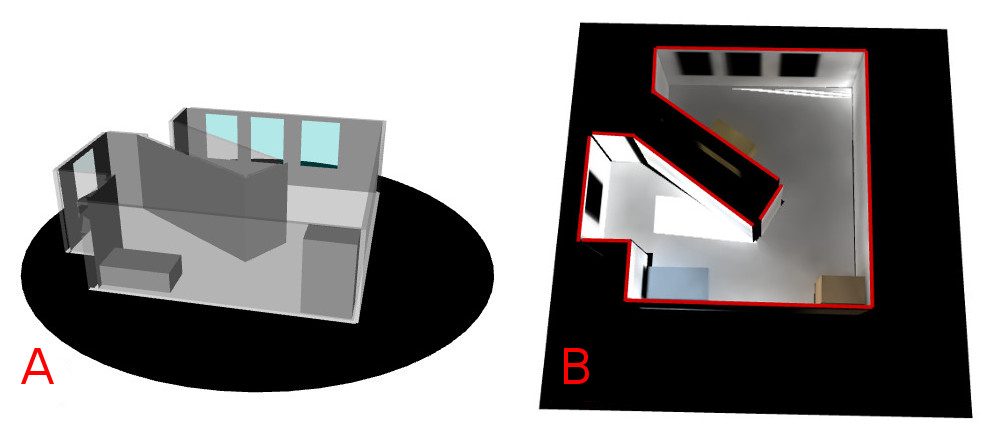
\includegraphics[width=0.8\textwidth]{viewer}
\caption{On the left is an example of the sketch interpretation viewer and on the right is an example of the daylight rendering viewer.}
\label{fig:viewer}
\end{figure}

\paragraph{Daylight Rendering Viewer}
The daylight rendering viewer is located on the \textit{Analyze Simulation} page. This viewer supports the same navigation controls as the sketch interpretation viewer. However, there are two visualization modes users can choose from on the daylight rendering viewer; this viewer supports daylight renderings and false color visualizations. These two visualization modes are illustrated in Figure-\ref{false_color}.
In Figure-\ref{false_color}B the false color visualization brings users attention to areas that suffer from over and under illumination. This feature was ported from the Virtual Heliodon and displays a textured checkerboard image on surfaces that fall below or above specific thresholds in relation to the daylight rendering engine's illumination values\cite{nasman2013evaluation}. Red checkerboard patterns are used to represent over illumination and blue checkerboard patterns for under illumination.Our intention as an early design tool is to have users analyze the daylight visualization results on the \textit{Analyze Simulation} page. From their analysis users are either satisfied with the distribution of daylight in their model or choose to make renovations. Improvements include making alterations to diffuse lighting if over illumination is a problem. Additionally, improvements could include making windows larger or changing the orientation of the room to make better use of daylight. Overall, the daylight rendering viewer should not be the final step on users' work flow in OASIS, but instead be a point of evaluation that communicates to users where problems lie so that they may go back and make edits to their design and continue the cycle of the creative iterative design process. 

\begin{figure}[h]
\centering
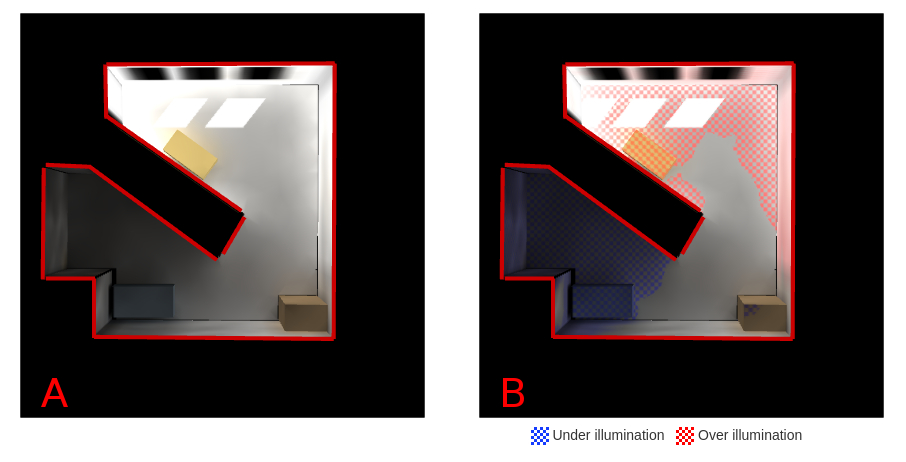
\includegraphics[width=0.8\textwidth]{false_color}
\caption{The two visualization modes of the daylight rendering viewer. On the left is a daylight rendering of a model and on the right is a false-color visualization of a model highlighting areas that suffer from over and under illumination.}
\label{fig:false_color}
\end{figure}

\paragraph{Share A Model Viewer}
Current work is being done on a \textit{Share A Model} viewer. This viewer would allow users to share models via generated URLS.The purpose of this viewer is two fold. Firstly, I suspect it would make sharing models between users much easier than sharing accounts or taking screenshots of OASIS and replicating sketches via tracing. In essence this feature would allow users to fork models from other users. Secondly, I hope this feature would allow users to share models between non-users, including family and friends. Rather than taking screenshots, non-users can visit the URL provided from a user and view the 3D rendering of a model without needing to sign up for an account. Figure-\ref{fig:share} illustrates the viewer in its current state. As mentioned, this stand alone viewer is currently under development.
\begin{figure}[h]
\centering
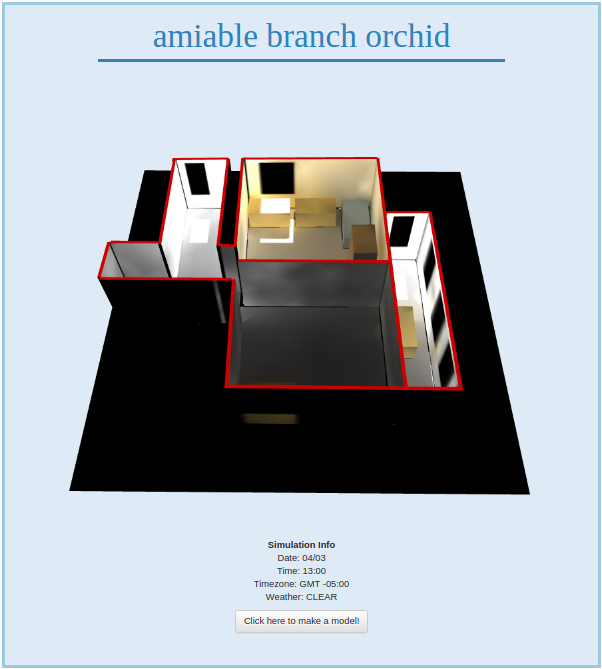
\includegraphics[width=0.8\textwidth]{share}
\caption{Share A Model viewer in its current state of development. No user registration is required to view a model.}
\label{fig:share}
\end{figure}

\section{General Web Application Design}

\paragraph{Ribbon Design Choice} As mentioned previously in section-\ref{ui_importance} the user interface of any tool is of great significance. 
For that reason I choose to use a ribbon interface to organize the pages and tools on OASIS. 
The Ribbon interface is common to contemporary Microsoft products and even a few other daylight analysis tools\cite{todo}.
The hope is that organizing tools and pages in an interface that might be familiar to users would make using OASIS easier. Figure-\ref{fig:ribbon} illustrates the similarities between our interface and Microsoft Word.


\begin{figure}[h]
\centering
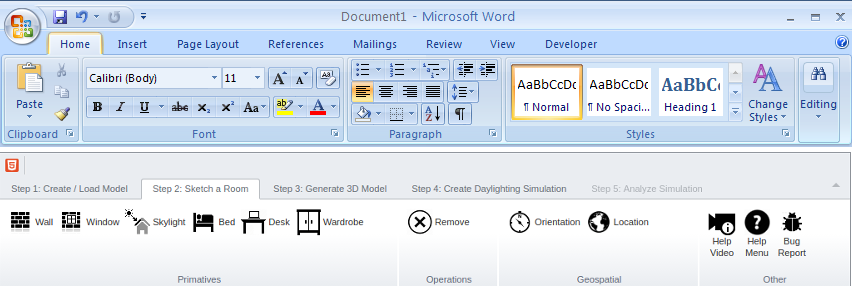
\includegraphics[width=1\textwidth]{ribbon}
\caption{On the top is Microsoft Word's ribbon and on the bottom is OASIS' version of a ribbon.}
\label{fig:ribbon}
\end{figure}


\paragraph{Nonlinear Navigation in OASIS}

% Non-Linearity in OASIS
% Loading Previous Models and Rendering Task

\paragraph{Problems Encountered}
% Computational Intensive Procedures
% Saving Models Safety
% Dealing with Clueless Users

\paragraph{Implementation}

\paragraph{Frameworks Used}

\paragraph{WebGL}

\paragraph{RaphaelJS}
Another framework used in our sketching interface is RaphaelJS\cite{todo}.
Raphael JS is a 3D vector graphics library for JavaScript. 
I use RaphaelJS to create 2D graphics of objects users places into sketches. I also use RaphaelJS because it supports vectorized lines and shapes, allowing our interface  to be re-sizable with lost of visual quality.
I also use Raphael FreeTransform in conjunction with RaphaelJS\cite{todo}. 
The FreeTransform extension is used to create FreeTransform handles on furniture items so that users may easily rotate and reposition furniture items where they please.
Figure-\ref{fig:oldvh}F demonstrates the handles FreeTransform generates for object manipulation.\\

\paragraph{RibbonJS}

\section{Chapter Summary}
% Summary of what we covered

